\section{Análise Exploratória de Dados (EDA)}

A primeira etapa do projeto consistiu em realizar uma análise exploratória sobre os dados de tráfego para
compreender suas características fundamentais.
O \emph{dataset} original, após ser processado, resultou em uma série temporal de volume de tráfego agregado
por segundo.

\begin{table}[!htb]
    \centering
    \caption{Estatísticas descritivas para a série temporal de \texttt{bytes\_per\_second}.}
    \label{tab:eda-describe}
    ../../results/200701251400.describe.tex
\end{table}

A \Cref{tab:eda-describe} apresenta as estatísticas descritivas da série.
[... Adicione seus comentários aqui sobre a média, desvio padrão, e a faixa de valores (min/max) ...]

\begin{figure}[!htb]
    \centering
    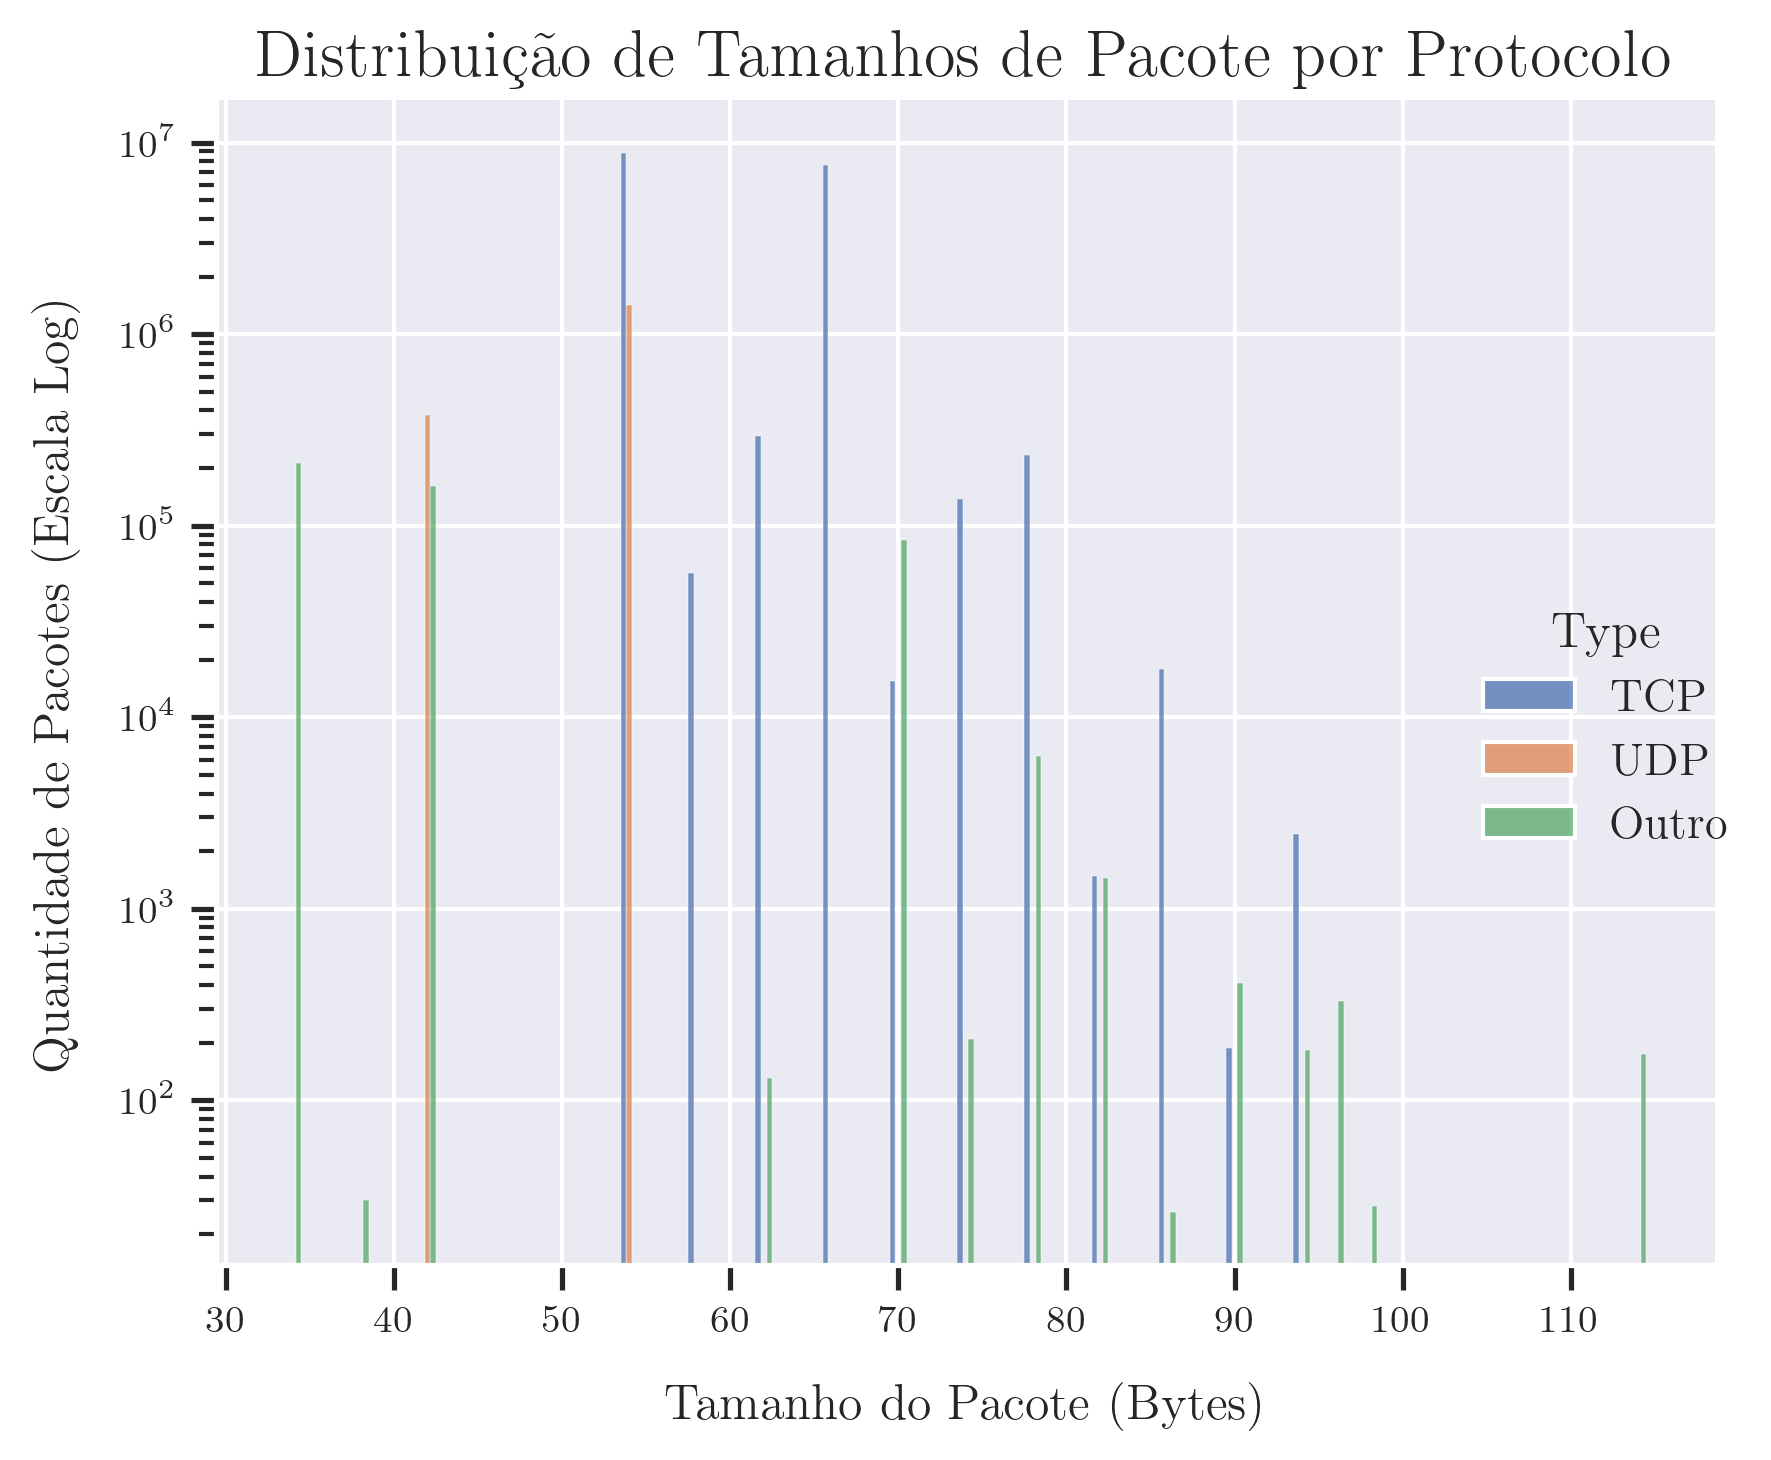
\includegraphics[width=0.95\textwidth]{resource/200701251400.protocol_dist.png}
    \caption{Distribuição de tamanhos de pacote para os protocolos TCP e UDP. A frequência (eixo Y) está em
    escala logarítmica para melhor visualização.}
    \label{fig:eda-protocol-dist}
\end{figure}

A \Cref{fig:eda-protocol-dist} ilustra a distribuição dos tamanhos de pacote.
[... Adicione seus comentários aqui, observando por exemplo os picos de pacotes pequenos (ACKs TCP) e grandes
(dados) ...]

\begin{figure}[!htb]
    \centering
    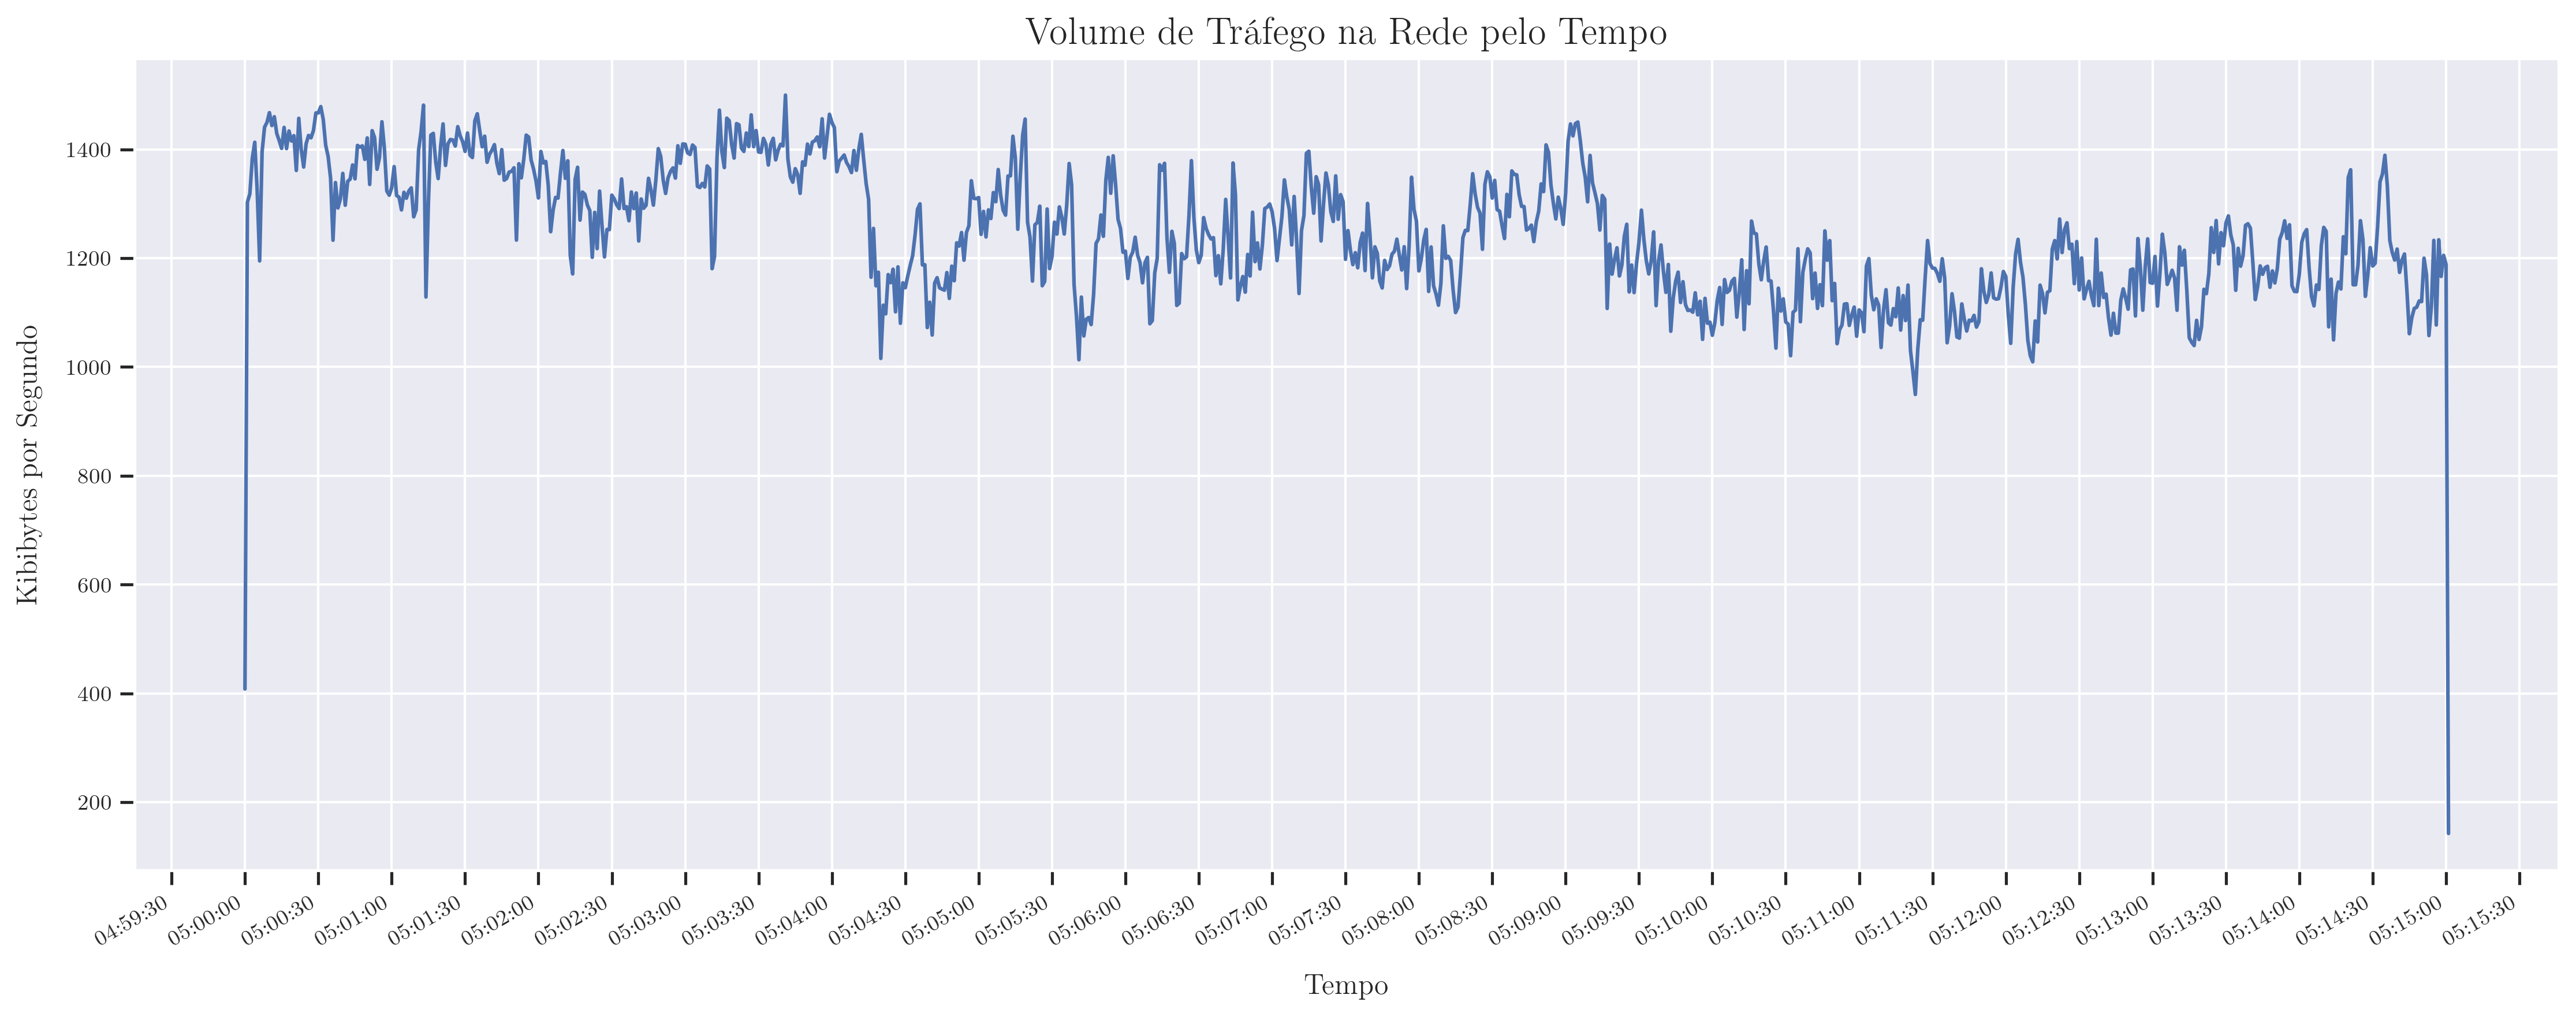
\includegraphics[width=0.95\textwidth]{resource/200701251400.time_series.png}
    \caption{Série temporal do volume de tráfego agregado por segundo.}
    \label{fig:eda-timeseries}
\end{figure}

A \Cref{fig:eda-timeseries} mostra o comportamento do tráfego ao longo do tempo.
[... Adicione seus comentários sobre a volatilidade, picos e períodos de estabilidade ...]

\begin{figure}[!htb]
    \centering
    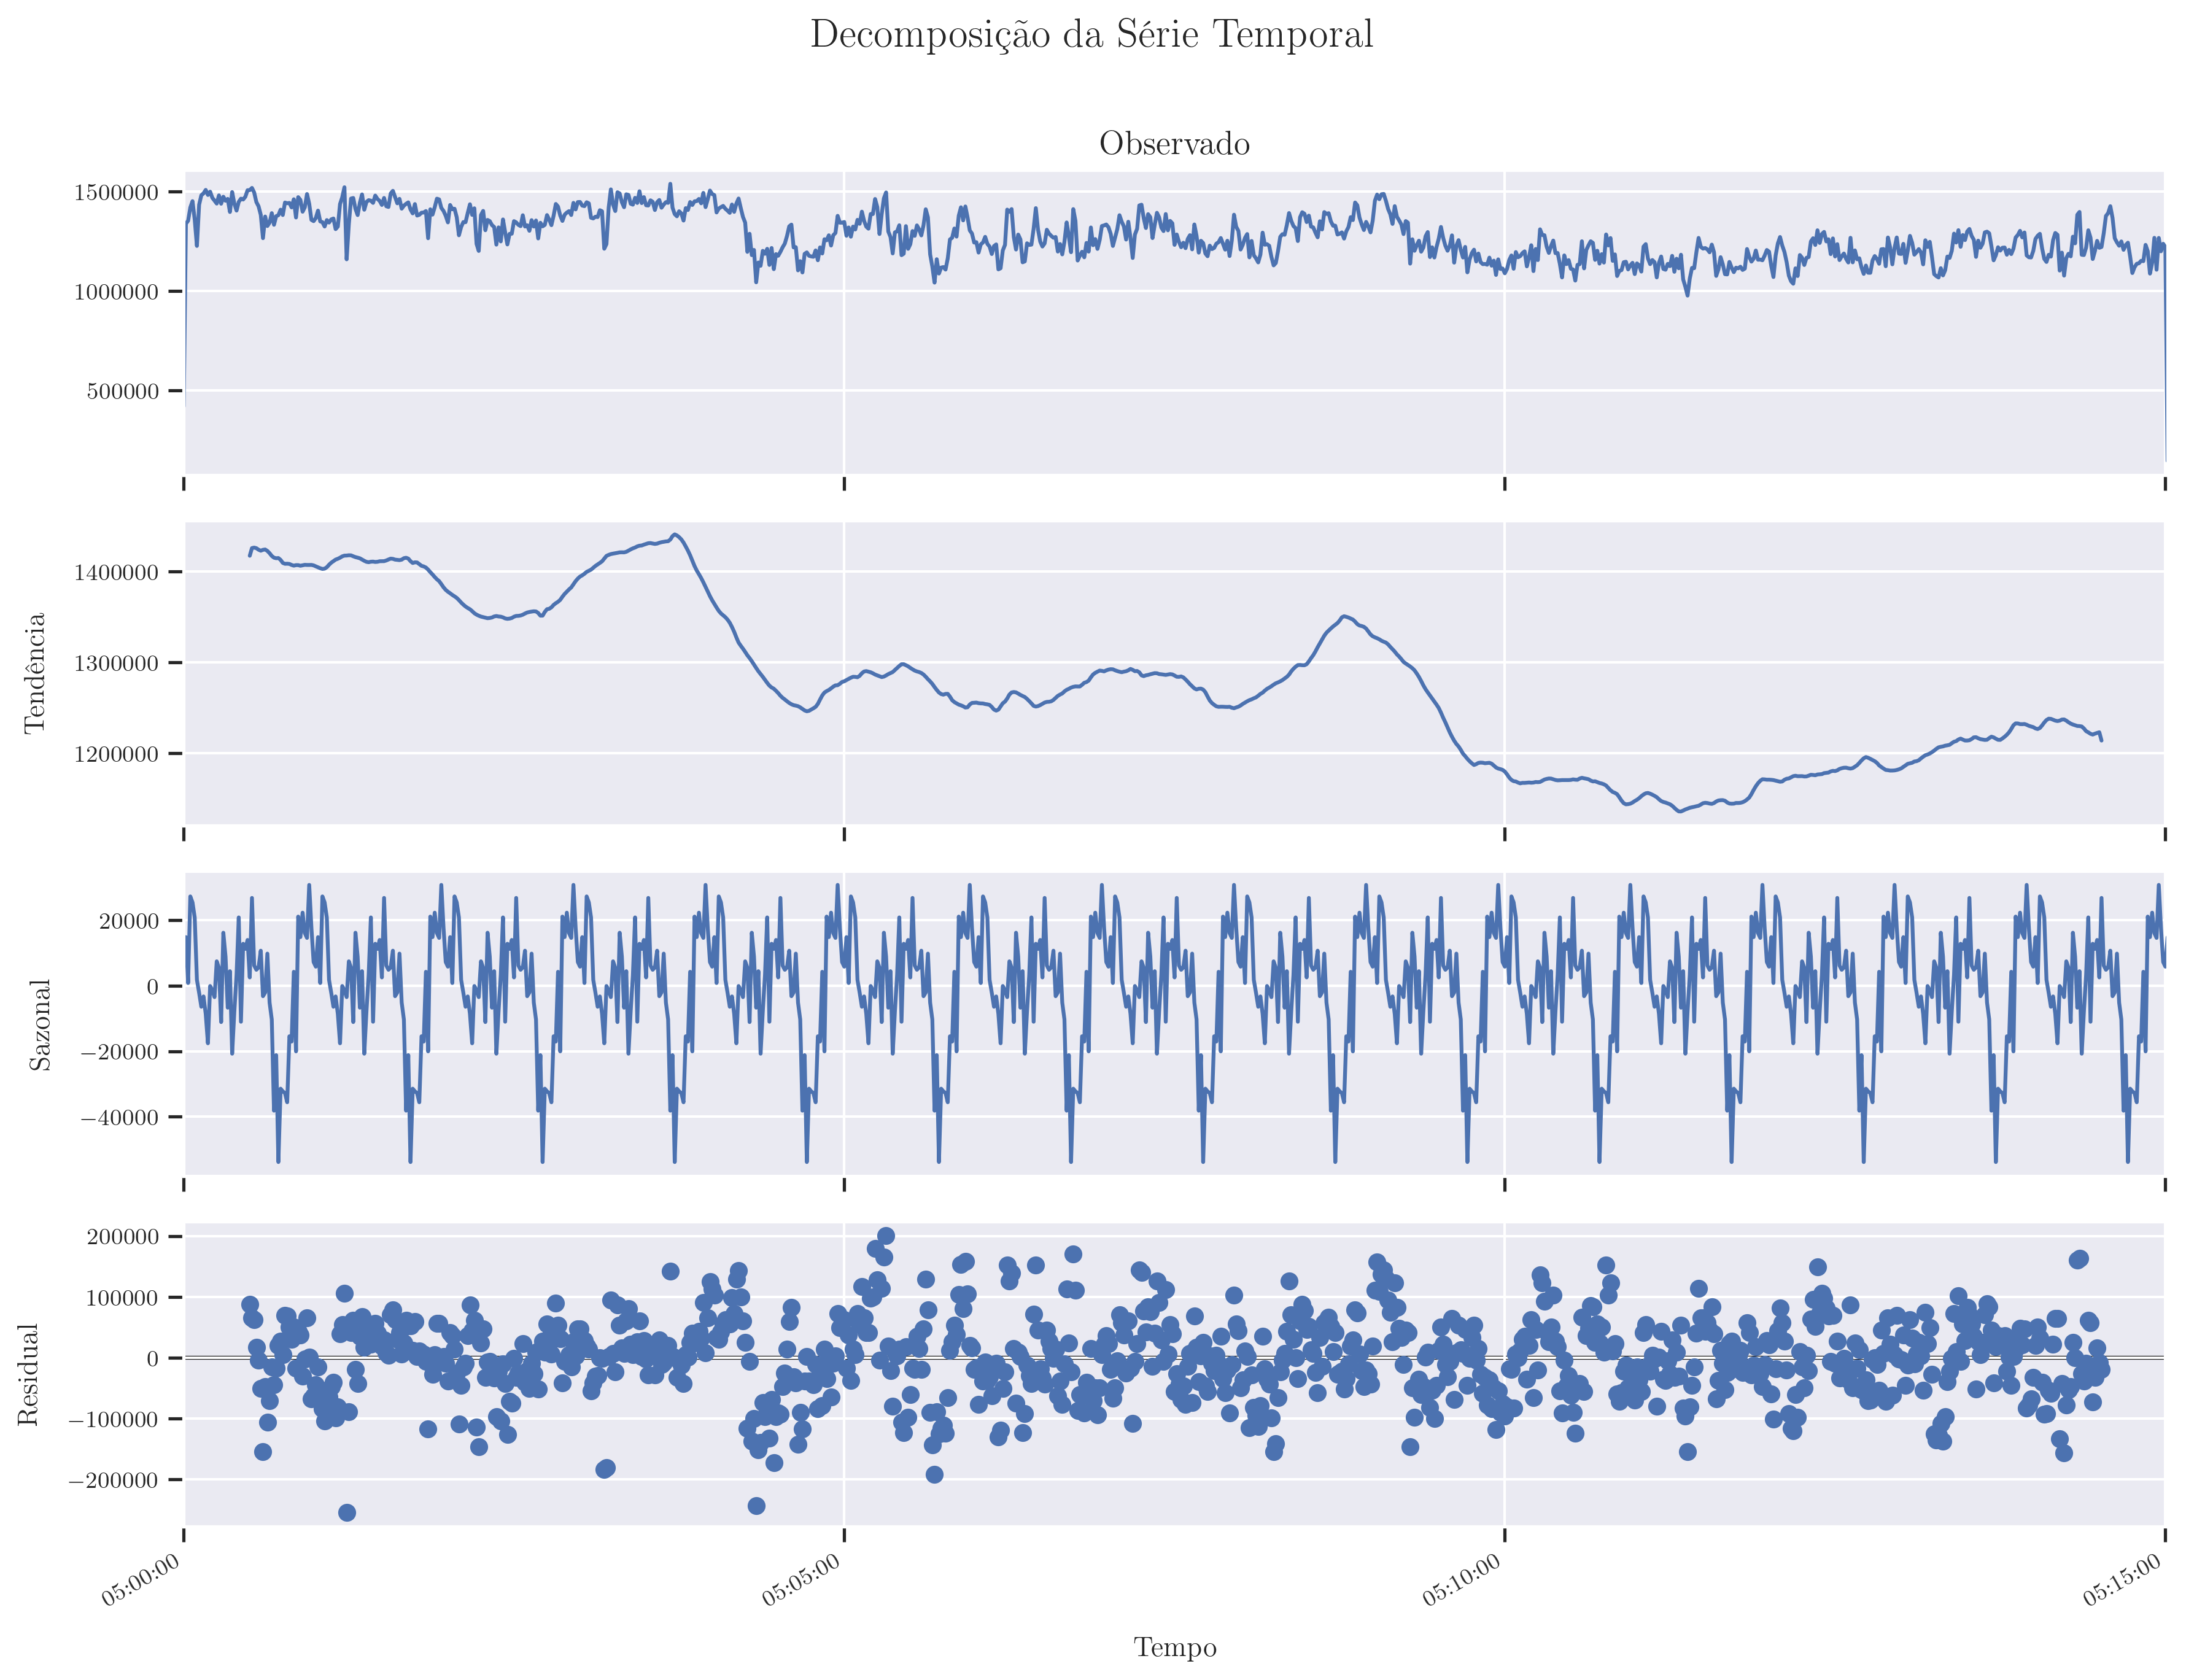
\includegraphics[width=0.8\textwidth]{resource/200701251400.decomposition.png}
    \caption{Decomposição da série temporal em tendência, sazonalidade e resíduos, com um período sazonal de
    60 segundos.}
    \label{fig:eda-decomposition}
\end{figure}

Para uma análise mais aprofundada, decompomos a série em seus componentes de tendência, sazonalidade e
resíduos, como visto na \Cref{fig:eda-decomposition}.
[... Adicione seus comentários sobre a tendência de longo prazo e os padrões periódicos (sazonais) que o
modelo precisará aprender ...]

\begin{figure}[!htb]
    \centering
    \includegraphics[width=0.7\textwidth]{resource/200701251400.autocorrelation.png}
    \caption{Funções de Autocorrelação (ACF) e Autocorrelação Parcial (PACF) para a série temporal.}
    \label{fig:eda-acf-pacf}
\end{figure}

Finalmente, a \Cref{fig:eda-acf-pacf} mostra as funções de autocorrelação. O decaimento lento da ACF confirma
a presença de uma forte tendência. A PACF, por sua vez, mostra correlações significativas nos primeiros lags,
justificando o uso de uma janela de look-back para o modelo LSTM.
[... Adicione seus comentários ...]
